
\documentclass[a4paper,12pt]{article}

\usepackage[a4paper, total={6in, 8in}, left=30mm]{geometry}
\usepackage{pdfpages}

\usepackage{cmap}
\usepackage[T2A]{fontenc}
\usepackage[utf8]{inputenc}
\usepackage[english,russian]{babel}
\usepackage{fancyhdr}
\usepackage{minted}
\usepackage{hyperref}
\usepackage{amsmath}
\usepackage{graphicx}

\hypersetup{
  pdfborderstyle={/S/U/W 1}
}

\graphicspath{{./images/}}

\pagestyle{fancy}
\fancyhf{}
\lhead{Антон Завьялов, ПИ-72}
\rhead{\textbf{Лабораторная №15, вариант 7}}
\cfoot{\thepage}

\makeatletter
\def\@seccntformat#1{
  \expandafter\ifx\csname c@#1\endcsname\c@section\else
  \csname the#1\endcsname\quad
  \fi}
\makeatother

\begin{document}
\includepdf[pages={1}]{title.pdf}

\section{\normalsize{Задание к лабораторной работе}}
\begin{flushleft}
  \textit{Постановка задачи}\linebreak
  Требуется найти приближенное значение решения следующей краевой задачи:

  \begin{equation}\label{eq:pos_1}
    \frac{d^2u(x)}{dx^2} + A(x)\frac{du(x)}{dx} + B(x)u(x) = C(x),~x \in [a,b],
  \end{equation}

  \begin{equation}\label{eq:pos_2}
    F_1u(a) + D_1\frac{du(a)}{dx} = E_1,
  \end{equation}

  \begin{equation}\label{eq:pos_2}
    F_2u(b) + D_2\frac{du(b)}{dx} = E_2.
  \end{equation}

  \textit{Задание к лабораторной работе}\linebreak
  \begin{itemize}
    \item По аналогии с описанным в параграфе 7.2 методом, вывести формулы для коэффициентов системы линейных алгебраических уравнений с трехдиагональной матрицей, которая получается для метода первого порядка аппроксимации.
    \item Составить программу для решения краевой задачи для линейного дифференциального уравнения второго порядка методом прогонки в случае первого и второго порядка аппроксимации.
    \item Провести вычисления, разбивая отрезок интегрирования на различное число частей, например, 25, 50, 100, 200.
    \item Проанализировать зависимость нормы разности между точным и приближенным решением от шага сетки для методов первого и второго порядка аппроксимации. Для этого составить таблицу или построить графики нормы разности для методов различного порядка аппроксимации. В качестве нормы можно взять C-норму. В этом случае норма функции равна максимальному значению модуля этой функции.
    \item Исследовать для Вашего варианта вопрос об устойчивости прогонки.
  \end{itemize}

  \textit{Для 7 варианта:}\linebreak
  \begin{equation}\label{eq:params}
    A(x) = \frac{4x}{2x+1}, B(x) = \frac{-4}{2x+1}, C(x) = 0,
  \end{equation}
  \begin{equation*}
    a = 0, b = 1,~F_1 = 1, D_1 = 1, E_1 = 0,~F_2 = 2, D_2 = 1, E_2 = 3,
  \end{equation*}
  \begin{equation*}
    u(x) = x + e^{-2x}.
  \end{equation*}
\end{flushleft}

\section{\normalsize{Краткое описание метода, расчётные формулы}}
\begin{flushleft}
  В методе $u', u'', ...$ выражаются численно через конечные разности на заданной равномерной сетке из $n$ частей $\{a,a+h, ..., b-h, b\}$, $h=\frac{b-a}{n}$.
  \linebreak\linebreak
  $u(x_i)$ обозначается как $y_i$, приводятся подобные и решается система $n$ линейных алгебраических уравнений.
  Т.к. в каждую конечную разность входят $y_{i-1, y_i, y_{i+1}}$, заданы значения $u$ на концах, можно решить систему методом прогонки.
  \linebreak\linebreak
  \textit{Система с трехдиагональной матрицей:}
  \begin{equation*}
    \left\{
      \begin{array}{lr}
          -b_0y_0 + c_0y_1 & = d_0,\\
        a_iy_{i-1} - b_iy_i + c_iy_{i+1} & = d_i, i = 1,...,n-1, \\
        a_ny_{n-1}-b_ny_n & = d_n.
      \end{array}
    \right.
  \end{equation*}
  \textit{Коэффициенты при первом порядке аппроксимации:}
  \begin{equation*}
    b_0 = -F_1h + D_1,~~c_0 = D_1,~~d_0=E_1h,
  \end{equation*}
  \begin{equation*}
    a_i = 1 - A(x_i)\frac{h}{2},~~b_i=2-B(x_i)h^2,~~c_i=1+A(x_i)\frac{h}{2},~~d_i=C(x_i)h^2,~i=1,...,n-1,
  \end{equation*}
  \begin{equation*}
    a_n=-D_2,~~b_n=-F_2h-D_2,~~d_n=E_2h.
  \end{equation*}
  \textit{Коэффициенты при втором порядке аппроксимации:}
  \begin{equation*}
    b_0 = -F_1h + D_1 + D_1(A(a)-B(a)h)\frac{h}{2},~~c_0 = A(a)D_1\frac{h}{2} + D_1,~~d_0=E_1h+C(a)D_1\frac{h^2}{2},
  \end{equation*}
  \begin{equation*}
    a_i = 1 - A(x_i)\frac{h}{2},~~b_i=2-B(x_i)h^2,~~c_i=1+A(x_i)\frac{h}{2},~~d_i=C(x_i)h^2,~i=1,...,n-1,
  \end{equation*}
  \begin{equation*}
    a_n=A(b)D_2\frac{h}{2}-D_2,~~b_n=-F_2h-D_2+D_2(A(b)+B(b)h)\frac{h}{2},~~d_n=E_2h-C(b)D_2\frac{h^2}{2}.
  \end{equation*}
\end{flushleft}


\section{\normalsize{Текст программы с комментариями}}
Кроме расположенных ниже листингов, исходный код можно посмотреть по адресу: \url{https://github.com/andiogenes/differential-equations/tree/master/finite-difference-method}
\linebreak\linebreak\textbf{Main.hs}
\inputminted[breaklines]{haskell}{../app/Main.hs}

\textbf{FiniteDifferenceMethod.hs}
\inputminted[breaklines]{haskell}{../src/FiniteDifferenceMethod.hs}

\textbf{Parameters.hs}
\inputminted[breaklines]{haskell}{../src/Parameters.hs}
\pagebreak

\section{\normalsize{Тестовые примеры}}
\begin{flushleft}
  \begin{itemize}
    \item При сетке из $n$ частей, $n=25$:\linebreak
      \includegraphics[scale=0.6]{solition_25.png}\linebreak
      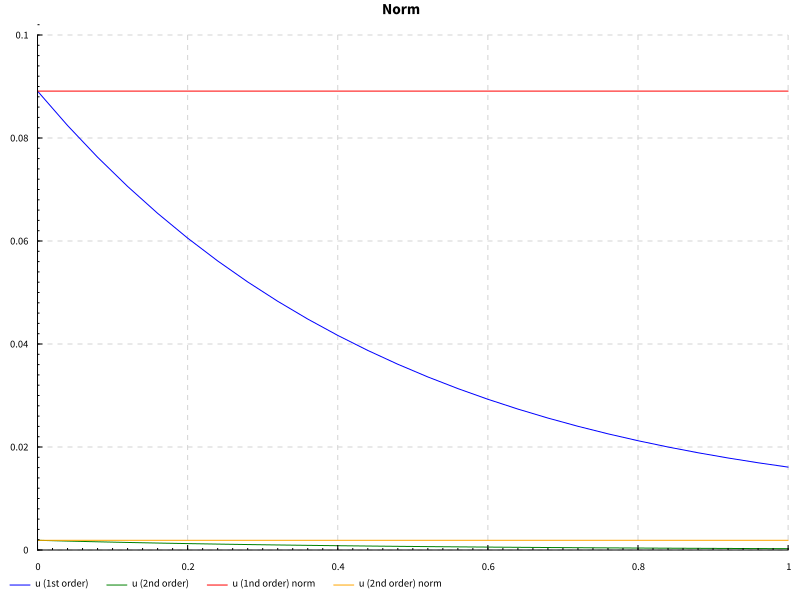
\includegraphics[scale=0.6]{norm_25.png}\linebreak
    \item $n=50$:\linebreak
      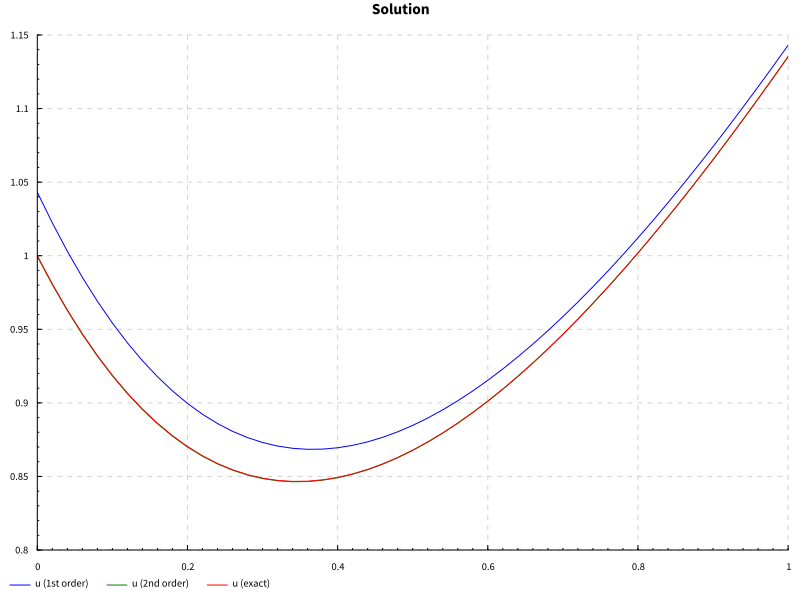
\includegraphics[scale=0.6]{solition_50.png}\linebreak
      \includegraphics[scale=0.6]{norm_50.png}\linebreak
    \item $n=100$:\linebreak
      \includegraphics[scale=0.6]{solution_100.png}\linebreak
      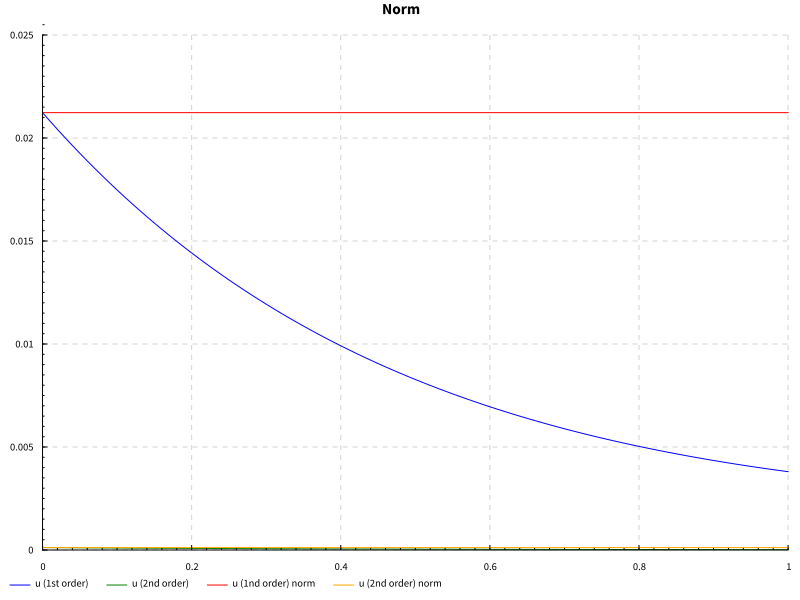
\includegraphics[scale=0.6]{norm_100.png}\linebreak
    \item $n=200$:\linebreak
      \includegraphics[scale=0.6]{solution_200.png}\linebreak
      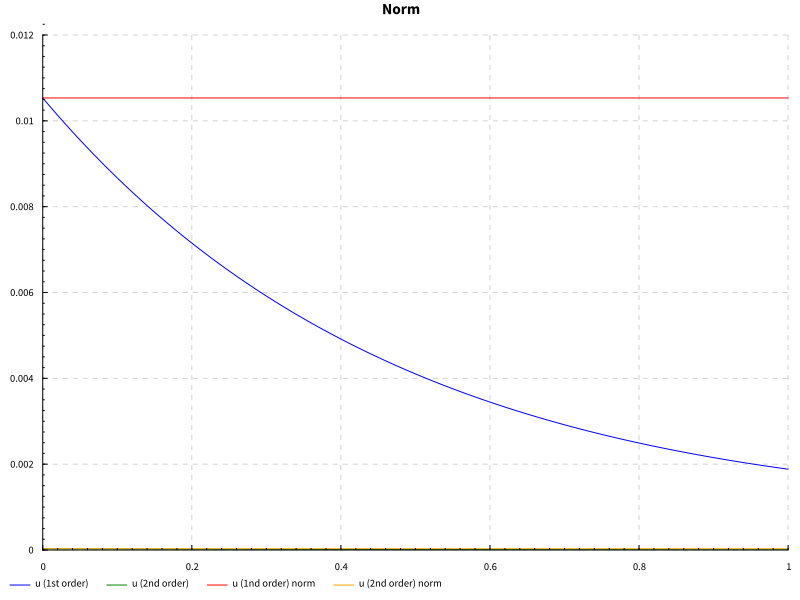
\includegraphics[scale=0.6]{norm_200.png}\linebreak
    \item $n=500$:\linebreak
      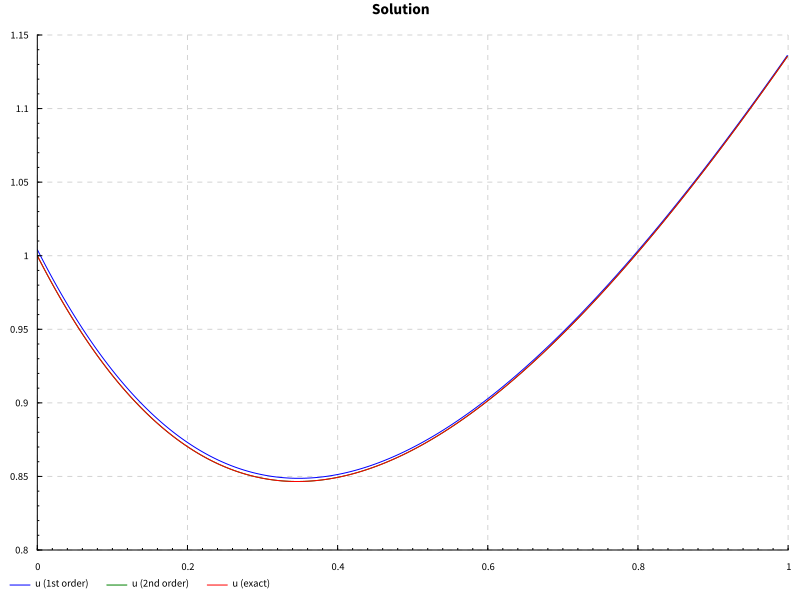
\includegraphics[scale=0.6]{solution_500.png}\linebreak
      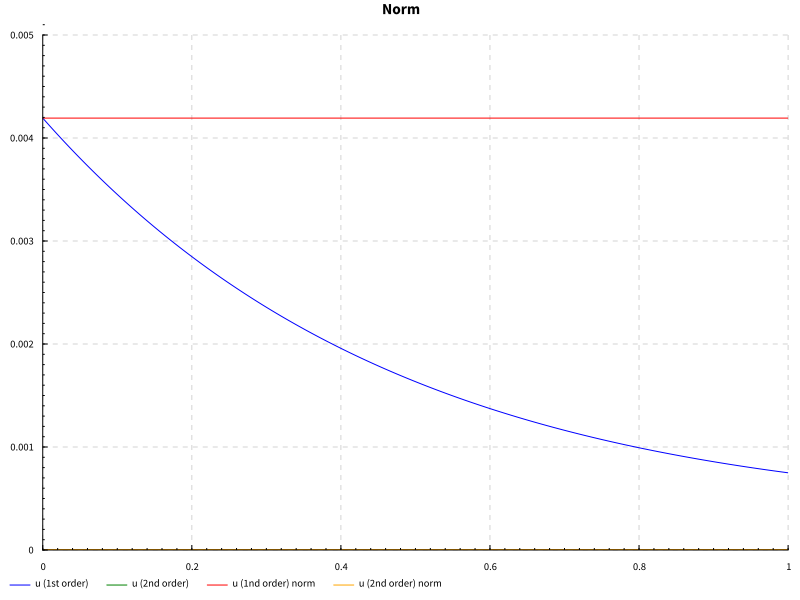
\includegraphics[scale=0.6]{norm_500.png}\linebreak
  \end{itemize}
\end{flushleft}
\begin{flushleft}
  По полученным результатам видно, что с увеличением $n$ оба решения стремятся к точному $u$.\linebreak\linebreak 
  При этом:
  \begin{itemize}
    \item Приближенное решение второго порядка аппроксимации сходится к $u$ на порядок быстрее, чем решение первого порядка;
    \item \(\mathopen| u_{approx}(x_1) - u(x_1) \mathclose| \le \mathopen| u_{approx}(x_2) - u(x_2) \mathclose|,~~x_1 \le x_2\);
    \item \(\displaystyle\max_x{\mathopen| u_{approx}(x) - u(x) \mathclose|} = \mathopen| u_{approx}(x_0) - u(x_0) \mathclose| \).
  \end{itemize}

  Последние два наблюдения объясняются накоплением погрешностей на прямом и обратном ходах метода прогонки.
\end{flushleft}

\section{\normalsize{Устойчивость прогонки}}
\begin{flushleft}
  \textit{Коэффициенты при первом порядке аппроксимации:}
  \begin{equation}\label{eq:koef11}
    b_0 = -h + 1,~~c_0 = 1,
  \end{equation}
  \begin{equation}\label{eq:koef12}
    a_i = 1 - \frac{4x_i}{2x_i+1}\frac{h}{2},~~b_i=2+\frac{4}{2x_i+1}h^2,~~c_i=1+\frac{4x_i}{2x_i+1}\frac{h}{2},~i=1,...,n-1,
  \end{equation}
  \begin{equation}\label{eq:koef13}
    a_n=-1,~~b_n=-2h-1.
  \end{equation}
  \textit{Коэффициенты при втором порядке аппроксимации:}
  \begin{equation}\label{eq:koef21}
    b_0 = -h + 1 + (\frac{4a}{2a+1}+\frac{4}{2a+1}h)\frac{h}{2},~~c_0 = \frac{4a}{2a+1}\frac{h}{2} + 1,
  \end{equation}
  \begin{equation}\label{eq:koef22}
    a_i = 1 - \frac{4x_i}{2x_i+1}\frac{h}{2},~~b_i=2+\frac{4}{2x_i+1}h^2,~~c_i=1+\frac{4x_i}{2x_i+1}\frac{h}{2},~i=1,...,n-1,
  \end{equation}
  \begin{equation}\label{eq:koef23}
    a_n=\frac{4b}{2b+1}\frac{h}{2}-1,~~b_n=-2h-1+(\frac{4b}{2b+1}-\frac{4}{2b+1}h)\frac{h}{2}.
  \end{equation}
  \textit{Условие диагонального преобладания}
  \begin{equation}\label{eq:diagsup}
    \mathopen| a_i \mathclose| > 0, \mathopen| c_i \mathclose| > 0, i = 2,...,m-1,
  \end{equation}
  \begin{equation*}
    \mathopen| b_i \mathclose| \ge \mathopen| a_i \mathclose| + \mathopen| c_i \mathclose|, i = 1, ...,m.
  \end{equation*}
\end{flushleft}
\begin{flushleft}
  Из \eqref{eq:koef11}, \eqref{eq:diagsup} диагональное преобладание нарушается, но при измельчении шага $b_o$ приближается слева к $c_0$.\linebreak\linebreak
  В \eqref{eq:koef12} $a_i, b_i, c_i$ неотрицательны на $[0,1]$, поэтому: \begin{enumerate}\item Выполняется первая часть \eqref{eq:diagsup}, \item В \eqref{eq:diagsup} можно опустить модули.\end{enumerate}
  \begin{equation*}
    2 + \frac{4}{2x_i+1}h^2 \ge 1 - \frac{4x_i}{2x_i+1}\frac{h}{2} + 1 + \frac{4x_i}{2x_i+1}\frac{h}{2},
  \end{equation*}
  \begin{equation*}
    \frac{4}{2x_i+1}h^2 \ge 0.
  \end{equation*}
  Очевидно, что это неравенство выполняется при любом $x_i \in [0,1],~h > 0$.\linebreak\linebreak
  Если в \eqref{eq:koef13} возьмём модули, получим:
  \begin{equation}\label{eq:k1c}
    2h+1 \ge 1 \implies 2h \ge 0.
  \end{equation}
  Таким образом, метод прогонки для трехдиагональной матрицы с коэффициентами \eqref{eq:koef11}, \eqref{eq:koef12}, \eqref{eq:koef13} строго говоря не является устойчивым из-за коэффициентов при $i=0$. \linebreak\linebreak
  Если в \eqref{eq:koef21} подставим $a=0$, получим выражения, аналогичные \eqref{eq:koef11}.\linebreak\linebreak\eqref{eq:koef12} и \eqref{eq:koef22} одинаковы.\linebreak\linebreak

  Подставив в \eqref{eq:koef23} $b=1$ получим:
  \begin{equation*}
    a_n = \frac{2h}{3} - 1, b_n = -\frac{4h}{3} - \frac{2h^2}{3} - 1,
  \end{equation*}
  \begin{equation*}
    \mathopen| a_n \mathclose| = 1 - \frac{2h}{3}, \mathopen| b_n \mathclose| = \frac{3 + 4h + 2h^2}{3}.
  \end{equation*}
  Далее в \eqref{eq:diagsup}:
  \begin{equation}\label{eq:k2c}
    \frac{3+4h+2h^2}{3} \ge \frac{3 - 2h}{3} \implies 2h^2 + 2h \ge 0.
  \end{equation}
  Очевидно, что это неравенство выполняется при $h > 0$. Заметим, что в сравнении с \eqref{eq:k1c}, \eqref{eq:k2c} имеет добавку $2h^2$.\linebreak\linebreak
  Для матрицы с коэффициентами \eqref{eq:koef21}, \eqref{eq:koef22}, \eqref{eq:koef23} метод прогонки не является устойчивым по той же причине, что и в предыдущем случае.\linebreak\linebreak
  Заметим также, если критерий устойчивости выражать как $\mathopen| \alpha_i \mathclose| \le 1, \forall i \in 0, ..., n$, он тоже не будет выполнен, так как $\alpha_1 = c_0/b_0 = 1/(1-h) > 1$.\linebreak

  
\end{flushleft}

\end{document}
